\documentclass{whiteboard}
\begin{document}
\begin{frame}[plain,t]
 \bbcover{SPOJ SUBMERGE}{Submerging Islands}{Prof. Edson Alves}{Faculdade UnB Gama}
\end{frame}

\begin{frame}[plain,t]
\vspace*{\fill}
 \bbenglish{Vice City is built over a group of islands, with bridges connecting them. As anyone in Vice City knows, the biggest fear of vice-citiers is that some day the islands will submerge. The big problem with this is that once the islands submerge, some of the other islands could get disconnected. You have been hired by the mayor of Vice city to tell him how many islands, when submerged, will disconnect parts of Vice City. You should know that initially all the islands of the city are connected.}
\vspace*{\fill}
\end{frame}

\begin{frame}[plain,t]
\vspace*{\fill}
 \bbtext{Vice City foi construída sobre um grupo de ilhas, com pontes conectando-as. Como todos em Vice City sabem, o maior medo dos moradores é que em algum dia as ilhas venham a submergir. O maior problema é que, uma vez que uma ilha afunde, as outras ilhas podem ficar desconectadas. Você foi contratado pelo prefeito de Vice City para dizer a ele quantas ilhas, se submergissem, desconectariam as ilhas de Vice City. Assuma que todas as ilhas da cidade estão inicialmente conectadas.}
\vspace*{\fill}
\end{frame}

\begin{frame}[plain,t]
\vspace*{\fill}
 \bbbold{Input}

 \vspace{0.1in}

 \bbenglish{The input will consist of a series of test cases. Each test case will start with the number $N$ $(1\leq N\leq 10^4)$ of islands, and the number $M$ of bridges $(1\leq M\leq 10^5)$. Following there will be $M$ lines each describing a bridge. Each of these M lines will contain two integers $U_i, V_i$ $(1\leq U_i, V_i\leq N)$, indicating that there is a bridge connecting islands $U_i$ and $V_i$. The input ends with a case where $N = M = 0$.}

 \vspace{0.2in}

 \bbbold{Output}

 \vspace{0.1in}

 \bbenglish{For each case on the input you must print a line indicating the number of islands that, when submerged, will disconnect parts of the city.}
\vspace*{\fill}
\end{frame}

\begin{frame}[plain,t]
\vspace*{\fill}
 \bbbold{Entrada}

 \vspace{0.1in}

 \bbtext{A entrada é composta por uma série de casos de teste. Cada caso de teste irá começar com o número $N$ $(1\leq N\leq 10^4)$ de ilhas e o número $M$ de pontes $(1\leq M\leq 10^5)$. Em seguida haverão $M$ linha, cada uma descrevendo uma ponte. Cada uma destas M linha conterá dois inteiros $U_i, V_i$ $(1\leq U_i, V_i\leq N)$, indicando que há uma ponte conectando as ilhas $U_i$ e $V_i$. A entrada termina com um caso de teste onde $N = M = 0$.}

 \vspace{0.2in}

 \bbbold{Saída}

 \vspace{0.1in}

 \bbtext{Para cada caso da entrada você deve imprimr uma linha indicando o número de ilhas que, se submergidas, desconectariam partes da cidade.}
\vspace*{\fill}
\end{frame}

\begin{frame}[plain,t]
\begin{tikzpicture}
\node[draw,opacity=0] at (0, 0) {x};
\node[draw,opacity=0] at (14, 8) {x};
 \node[anchor=west] at (0, 7) { \bbbold{Exemplo de entrada e saída} };
\end{tikzpicture}
\end{frame}

\begin{frame}[plain,t]
\begin{tikzpicture}
\node[draw,opacity=0] at (0, 0) {x};
\node[draw,opacity=0] at (14, 8) {x};
 \node[anchor=west] at (0, 7) { \bbbold{Exemplo de entrada e saída} };
 \node[anchor=west] at (1, 6) { \bbtext{3 3} };
\end{tikzpicture}
\end{frame}

\begin{frame}[plain,t]
\begin{tikzpicture}
\node[draw,opacity=0] at (0, 0) {x};
\node[draw,opacity=0] at (14, 8) {x};
 \node[anchor=west] at (0, 7) { \bbbold{Exemplo de entrada e saída} };
 \node[anchor=west] at (1, 6) { \bbtext{3 3} };
 \node[anchor=west] at (0.5, 5) { \footnotesize \bbcomment{\# de ilhas} };
 \draw[->,color=BBViolet] (1.25, 5.2) -- (1.25, 5.8);
\end{tikzpicture}
\end{frame}

\begin{frame}[plain,t]
\begin{tikzpicture}
\node[draw,opacity=0] at (0, 0) {x};
\node[draw,opacity=0] at (14, 8) {x};
 \node[anchor=west] at (0, 7) { \bbbold{Exemplo de entrada e saída} };
 \node[anchor=west] at (1, 6) { \bbtext{3 3} };
 \node[anchor=west] at (0.5, 5) { \footnotesize \bbcomment{\# de ilhas} };
 \draw[->,color=BBViolet] (1.25, 5.2) -- (1.25, 5.8);
 \node[anchor=west] at (2.9, 6) { \footnotesize \bbcomment{\# de pontes} };
 \draw[->,color=BBViolet] (1.8, 6) -- (2.8, 6);
\end{tikzpicture}
\end{frame}

\begin{frame}[plain,t]
\begin{tikzpicture}
\node[draw,opacity=0] at (0, 0) {x};
\node[draw,opacity=0] at (14, 8) {x};
 \node[anchor=west] at (0, 7) { \bbbold{Exemplo de entrada e saída} };
 \node[anchor=west] at (1, 6) { \bbtext{3 3} };
 \node[circle,draw,very thick] (A) at (6, 2) { \bbtext{1} };
 \node[circle,draw,very thick] (B) at (9, 6) { \bbtext{2} };
 \node[circle,draw,very thick] (C) at (12, 2) { \bbtext{3} };
\end{tikzpicture}
\end{frame}

\begin{frame}[plain,t]
\begin{tikzpicture}
\node[draw,opacity=0] at (0, 0) {x};
\node[draw,opacity=0] at (14, 8) {x};
 \node[anchor=west] at (0, 7) { \bbbold{Exemplo de entrada e saída} };
 \node[anchor=west] at (1, 6) { \bbtext{3 3} };
 \node[circle,draw,very thick] (A) at (6, 2) { \bbtext{1} };
 \node[circle,draw,very thick] (B) at (9, 6) { \bbtext{2} };
 \node[circle,draw,very thick] (C) at (12, 2) { \bbtext{3} };
 \node[anchor=west] at (1, 5.5) { \bbtext{1 2} };
\end{tikzpicture}
\end{frame}

\begin{frame}[plain,t]
\begin{tikzpicture}
\node[draw,opacity=0] at (0, 0) {x};
\node[draw,opacity=0] at (14, 8) {x};
 \node[anchor=west] at (0, 7) { \bbbold{Exemplo de entrada e saída} };
 \node[anchor=west] at (1, 6) { \bbtext{3 3} };
 \node[circle,draw,very thick] (A) at (6, 2) { \bbtext{1} };
 \node[circle,draw,very thick] (B) at (9, 6) { \bbtext{2} };
 \node[circle,draw,very thick] (C) at (12, 2) { \bbtext{3} };
 \node[anchor=west] at (1, 5.5) { \bbtext{1 2} };
 \draw[very thick] (A) to (B);
\end{tikzpicture}
\end{frame}

\begin{frame}[plain,t]
\begin{tikzpicture}
\node[draw,opacity=0] at (0, 0) {x};
\node[draw,opacity=0] at (14, 8) {x};
 \node[anchor=west] at (0, 7) { \bbbold{Exemplo de entrada e saída} };
 \node[anchor=west] at (1, 6) { \bbtext{3 3} };
 \node[circle,draw,very thick] (A) at (6, 2) { \bbtext{1} };
 \node[circle,draw,very thick] (B) at (9, 6) { \bbtext{2} };
 \node[circle,draw,very thick] (C) at (12, 2) { \bbtext{3} };
 \node[anchor=west] at (1, 5.5) { \bbtext{1 2} };
 \draw[very thick] (A) to (B);
 \node[anchor=west] at (1, 5.0) { \bbtext{2 3} };
\end{tikzpicture}
\end{frame}

\begin{frame}[plain,t]
\begin{tikzpicture}
\node[draw,opacity=0] at (0, 0) {x};
\node[draw,opacity=0] at (14, 8) {x};
 \node[anchor=west] at (0, 7) { \bbbold{Exemplo de entrada e saída} };
 \node[anchor=west] at (1, 6) { \bbtext{3 3} };
 \node[circle,draw,very thick] (A) at (6, 2) { \bbtext{1} };
 \node[circle,draw,very thick] (B) at (9, 6) { \bbtext{2} };
 \node[circle,draw,very thick] (C) at (12, 2) { \bbtext{3} };
 \node[anchor=west] at (1, 5.5) { \bbtext{1 2} };
 \draw[very thick] (A) to (B);
 \node[anchor=west] at (1, 5.0) { \bbtext{2 3} };
 \draw[very thick] (B) to (C);
\end{tikzpicture}
\end{frame}

\begin{frame}[plain,t]
\begin{tikzpicture}
\node[draw,opacity=0] at (0, 0) {x};
\node[draw,opacity=0] at (14, 8) {x};
 \node[anchor=west] at (0, 7) { \bbbold{Exemplo de entrada e saída} };
 \node[anchor=west] at (1, 6) { \bbtext{3 3} };
 \node[circle,draw,very thick] (A) at (6, 2) { \bbtext{1} };
 \node[circle,draw,very thick] (B) at (9, 6) { \bbtext{2} };
 \node[circle,draw,very thick] (C) at (12, 2) { \bbtext{3} };
 \node[anchor=west] at (1, 5.5) { \bbtext{1 2} };
 \draw[very thick] (A) to (B);
 \node[anchor=west] at (1, 5.0) { \bbtext{2 3} };
 \draw[very thick] (B) to (C);
 \node[anchor=west] at (1, 4.5) { \bbtext{1 3} };
\end{tikzpicture}
\end{frame}

\begin{frame}[plain,t]
\begin{tikzpicture}
\node[draw,opacity=0] at (0, 0) {x};
\node[draw,opacity=0] at (14, 8) {x};
 \node[anchor=west] at (0, 7) { \bbbold{Exemplo de entrada e saída} };
 \node[anchor=west] at (1, 6) { \bbtext{3 3} };
 \node[circle,draw,very thick] (A) at (6, 2) { \bbtext{1} };
 \node[circle,draw,very thick] (B) at (9, 6) { \bbtext{2} };
 \node[circle,draw,very thick] (C) at (12, 2) { \bbtext{3} };
 \node[anchor=west] at (1, 5.5) { \bbtext{1 2} };
 \draw[very thick] (A) to (B);
 \node[anchor=west] at (1, 5.0) { \bbtext{2 3} };
 \draw[very thick] (B) to (C);
 \node[anchor=west] at (1, 4.5) { \bbtext{1 3} };
 \draw[very thick] (A) to (C);
\end{tikzpicture}
\end{frame}

\begin{frame}[plain,t]
\begin{tikzpicture}
\node[draw,opacity=0] at (0, 0) {x};
\node[draw,opacity=0] at (14, 8) {x};
 \node[anchor=west] at (0, 7) { \bbbold{Exemplo de entrada e saída} };
 \node[anchor=west] at (1, 6) { \bbtext{3 3} };
 \node[circle,draw,very thick] (B) at (9, 6) { \bbtext{2} };
 \node[circle,draw,very thick] (C) at (12, 2) { \bbtext{3} };
 \node[anchor=west] at (1, 5.5) { \bbtext{1 2} };
 \draw[very thick] (A) to (B);
 \node[anchor=west] at (1, 5.0) { \bbtext{2 3} };
 \draw[very thick] (B) to (C);
 \node[anchor=west] at (1, 4.5) { \bbtext{1 3} };
 \draw[very thick] (A) to (C);
 \node[circle,fill,color=BBRed] (A) at (6, 2) { \bbtext{1} };
 \node[circle,draw,very thick] (A) at (6, 2) { \bbtext{1} };
\end{tikzpicture}
\end{frame}

\begin{frame}[plain,t]
\begin{tikzpicture}
\node[draw,opacity=0] at (0, 0) {x};
\node[draw,opacity=0] at (14, 8) {x};
 \node[anchor=west] at (0, 7) { \bbbold{Exemplo de entrada e saída} };
 \node[anchor=west] at (1, 6) { \bbtext{3 3} };
 \node[circle,draw,very thick] (B) at (9, 6) { \bbtext{2} };
 \node[circle,draw,very thick] (C) at (12, 2) { \bbtext{3} };
 \node[anchor=west] at (1, 5.5) { \bbtext{1 2} };
 \node[anchor=west] at (1, 5.0) { \bbtext{2 3} };
 \draw[very thick] (B) to (C);
 \node[anchor=west] at (1, 4.5) { \bbtext{1 3} };
\end{tikzpicture}
\end{frame}

\begin{frame}[plain,t]
\begin{tikzpicture}
\node[draw,opacity=0] at (0, 0) {x};
\node[draw,opacity=0] at (14, 8) {x};
 \node[anchor=west] at (0, 7) { \bbbold{Exemplo de entrada e saída} };
 \node[anchor=west] at (1, 6) { \bbtext{3 3} };
 \node[circle,draw,very thick] (B) at (9, 6) { \bbtext{2} };
 \node[circle,draw,very thick] (C) at (12, 2) { \bbtext{3} };
 \node[anchor=west] at (1, 5.5) { \bbtext{1 2} };
 \node[anchor=west] at (1, 5.0) { \bbtext{2 3} };
 \draw[very thick] (B) to (C);
 \node[anchor=west] at (1, 4.5) { \bbtext{1 3} };
 \node[circle,draw,very thick] (A) at (6, 2) { \bbtext{1} };
 \draw[very thick] (A) to (B);
 \draw[very thick] (A) to (C);
\end{tikzpicture}
\end{frame}

\begin{frame}[plain,t]
\begin{tikzpicture}
\node[draw,opacity=0] at (0, 0) {x};
\node[draw,opacity=0] at (14, 8) {x};
 \node[anchor=west] at (0, 7) { \bbbold{Exemplo de entrada e saída} };
 \node[anchor=west] at (1, 6) { \bbtext{3 3} };
 \node[circle,draw,very thick] (C) at (12, 2) { \bbtext{3} };
 \node[anchor=west] at (1, 5.5) { \bbtext{1 2} };
 \node[anchor=west] at (1, 5.0) { \bbtext{2 3} };
 \draw[very thick] (B) to (C);
 \node[anchor=west] at (1, 4.5) { \bbtext{1 3} };
 \node[circle,draw,very thick] (A) at (6, 2) { \bbtext{1} };
 \draw[very thick] (A) to (B);
 \draw[very thick] (A) to (C);
 \node[circle,fill,color=BBRed] (B) at (9, 6) { \bbtext{2} };
 \node[circle,draw,very thick] (B) at (9, 6) { \bbtext{2} };
\end{tikzpicture}
\end{frame}

\begin{frame}[plain,t]
\begin{tikzpicture}
\node[draw,opacity=0] at (0, 0) {x};
\node[draw,opacity=0] at (14, 8) {x};
 \node[anchor=west] at (0, 7) { \bbbold{Exemplo de entrada e saída} };
 \node[anchor=west] at (1, 6) { \bbtext{3 3} };
 \node[circle,draw,very thick] (C) at (12, 2) { \bbtext{3} };
 \node[anchor=west] at (1, 5.5) { \bbtext{1 2} };
 \node[anchor=west] at (1, 5.0) { \bbtext{2 3} };
 \node[anchor=west] at (1, 4.5) { \bbtext{1 3} };
 \node[circle,draw,very thick] (A) at (6, 2) { \bbtext{1} };
 \draw[very thick] (A) to (C);
\end{tikzpicture}
\end{frame}

\begin{frame}[plain,t]
\begin{tikzpicture}
\node[draw,opacity=0] at (0, 0) {x};
\node[draw,opacity=0] at (14, 8) {x};
 \node[anchor=west] at (0, 7) { \bbbold{Exemplo de entrada e saída} };
 \node[anchor=west] at (1, 6) { \bbtext{3 3} };
 \node[circle,draw,very thick] (C) at (12, 2) { \bbtext{3} };
 \node[anchor=west] at (1, 5.5) { \bbtext{1 2} };
 \node[anchor=west] at (1, 5.0) { \bbtext{2 3} };
 \node[anchor=west] at (1, 4.5) { \bbtext{1 3} };
 \node[circle,draw,very thick] (A) at (6, 2) { \bbtext{1} };
 \draw[very thick] (A) to (C);
 \node[circle,draw,very thick] (B) at (9, 6) { \bbtext{2} };
 \draw[very thick] (A) to (B);
 \draw[very thick] (B) to (C);
\end{tikzpicture}
\end{frame}

\begin{frame}[plain,t]
\begin{tikzpicture}
\node[draw,opacity=0] at (0, 0) {x};
\node[draw,opacity=0] at (14, 8) {x};
 \node[anchor=west] at (0, 7) { \bbbold{Exemplo de entrada e saída} };
 \node[anchor=west] at (1, 6) { \bbtext{3 3} };
 \node[anchor=west] at (1, 5.5) { \bbtext{1 2} };
 \node[anchor=west] at (1, 5.0) { \bbtext{2 3} };
 \node[anchor=west] at (1, 4.5) { \bbtext{1 3} };
 \node[circle,draw,very thick] (A) at (6, 2) { \bbtext{1} };
 \draw[very thick] (A) to (C);
 \node[circle,draw,very thick] (B) at (9, 6) { \bbtext{2} };
 \draw[very thick] (A) to (B);
 \draw[very thick] (B) to (C);
 \node[circle,fill,color=BBRed] (C) at (12, 2) { \bbtext{3} };
 \node[circle,draw,very thick] (C) at (12, 2) { \bbtext{3} };
\end{tikzpicture}
\end{frame}

\begin{frame}[plain,t]
\begin{tikzpicture}
\node[draw,opacity=0] at (0, 0) {x};
\node[draw,opacity=0] at (14, 8) {x};
 \node[anchor=west] at (0, 7) { \bbbold{Exemplo de entrada e saída} };
 \node[anchor=west] at (1, 6) { \bbtext{3 3} };
 \node[anchor=west] at (1, 5.5) { \bbtext{1 2} };
 \node[anchor=west] at (1, 5.0) { \bbtext{2 3} };
 \node[anchor=west] at (1, 4.5) { \bbtext{1 3} };
 \node[circle,draw,very thick] (A) at (6, 2) { \bbtext{1} };
 \node[circle,draw,very thick] (B) at (9, 6) { \bbtext{2} };
 \draw[very thick] (A) to (B);
\end{tikzpicture}
\end{frame}

\begin{frame}[plain,t]
\begin{tikzpicture}
\node[draw,opacity=0] at (0, 0) {x};
\node[draw,opacity=0] at (14, 8) {x};
 \node[anchor=west] at (0, 7) { \bbbold{Exemplo de entrada e saída} };
 \node[anchor=west] at (1, 6) { \bbtext{3 3} };
 \node[anchor=west] at (1, 5.5) { \bbtext{1 2} };
 \node[anchor=west] at (1, 5.0) { \bbtext{2 3} };
 \node[anchor=west] at (1, 4.5) { \bbtext{1 3} };
 \node[circle,draw,very thick] (A) at (6, 2) { \bbtext{1} };
 \node[circle,draw,very thick] (B) at (9, 6) { \bbtext{2} };
 \draw[very thick] (A) to (B);
 \node[circle,draw,very thick] (C) at (12, 2) { \bbtext{3} };
 \draw[very thick] (B) to (C);
 \draw[very thick] (A) to (C);
 \draw[-latex,very thick] (1.4, 3.2) to (1.4, 4.2);
 \node at (1.4, 2.9) { \bbinfo{0} };
\end{tikzpicture}
\end{frame}

\begin{frame}[plain,t]
\begin{tikzpicture}
\node[draw,opacity=0] at (0, 0) {x};
\node[draw,opacity=0] at (14, 8) {x};
 \node[anchor=west] at (0, 7) { \bbbold{Exemplo de entrada e saída} };
\end{tikzpicture}
\end{frame}

\begin{frame}[plain,t]
\begin{tikzpicture}
\node[draw,opacity=0] at (0, 0) {x};
\node[draw,opacity=0] at (14, 8) {x};
 \node[anchor=west] at (0, 7) { \bbbold{Exemplo de entrada e saída} };
 \node[anchor=west] at (1, 6) { \bbtext{6 8} };
\end{tikzpicture}
\end{frame}

\begin{frame}[plain,t]
\begin{tikzpicture}
\node[draw,opacity=0] at (0, 0) {x};
\node[draw,opacity=0] at (14, 8) {x};
 \node[anchor=west] at (0, 7) { \bbbold{Exemplo de entrada e saída} };
 \node[anchor=west] at (1, 6) { \bbtext{6 8} };
 \node[circle,draw,very thick] (A) at (6, 5) { \bbtext{1} };
 \node[circle,draw,very thick] (B) at (9, 7) { \bbtext{2} };
 \node[circle,draw,very thick] (C) at (12, 5) { \bbtext{3} };
 \node[circle,draw,very thick] (D) at (12, 3) { \bbtext{4} };
 \node[circle,draw,very thick] (E) at (9, 1) { \bbtext{5} };
 \node[circle,draw,very thick] (F) at (6, 3) { \bbtext{6} };
\end{tikzpicture}
\end{frame}

\begin{frame}[plain,t]
\begin{tikzpicture}
\node[draw,opacity=0] at (0, 0) {x};
\node[draw,opacity=0] at (14, 8) {x};
 \node[anchor=west] at (0, 7) { \bbbold{Exemplo de entrada e saída} };
 \node[anchor=west] at (1, 6) { \bbtext{6 8} };
 \node[circle,draw,very thick] (A) at (6, 5) { \bbtext{1} };
 \node[circle,draw,very thick] (B) at (9, 7) { \bbtext{2} };
 \node[circle,draw,very thick] (C) at (12, 5) { \bbtext{3} };
 \node[circle,draw,very thick] (D) at (12, 3) { \bbtext{4} };
 \node[circle,draw,very thick] (E) at (9, 1) { \bbtext{5} };
 \node[circle,draw,very thick] (F) at (6, 3) { \bbtext{6} };
 \node[anchor=west] at (1, 5.5) { \bbtext{1 3} };
\end{tikzpicture}
\end{frame}

\begin{frame}[plain,t]
\begin{tikzpicture}
\node[draw,opacity=0] at (0, 0) {x};
\node[draw,opacity=0] at (14, 8) {x};
 \node[anchor=west] at (0, 7) { \bbbold{Exemplo de entrada e saída} };
 \node[anchor=west] at (1, 6) { \bbtext{6 8} };
 \node[circle,draw,very thick] (A) at (6, 5) { \bbtext{1} };
 \node[circle,draw,very thick] (B) at (9, 7) { \bbtext{2} };
 \node[circle,draw,very thick] (C) at (12, 5) { \bbtext{3} };
 \node[circle,draw,very thick] (D) at (12, 3) { \bbtext{4} };
 \node[circle,draw,very thick] (E) at (9, 1) { \bbtext{5} };
 \node[circle,draw,very thick] (F) at (6, 3) { \bbtext{6} };
 \node[anchor=west] at (1, 5.5) { \bbtext{1 3} };
 \draw[very thick] (A) to (C);
\end{tikzpicture}
\end{frame}

\begin{frame}[plain,t]
\begin{tikzpicture}
\node[draw,opacity=0] at (0, 0) {x};
\node[draw,opacity=0] at (14, 8) {x};
 \node[anchor=west] at (0, 7) { \bbbold{Exemplo de entrada e saída} };
 \node[anchor=west] at (1, 6) { \bbtext{6 8} };
 \node[circle,draw,very thick] (A) at (6, 5) { \bbtext{1} };
 \node[circle,draw,very thick] (B) at (9, 7) { \bbtext{2} };
 \node[circle,draw,very thick] (C) at (12, 5) { \bbtext{3} };
 \node[circle,draw,very thick] (D) at (12, 3) { \bbtext{4} };
 \node[circle,draw,very thick] (E) at (9, 1) { \bbtext{5} };
 \node[circle,draw,very thick] (F) at (6, 3) { \bbtext{6} };
 \node[anchor=west] at (1, 5.5) { \bbtext{1 3} };
 \draw[very thick] (A) to (C);
 \node[anchor=west] at (1, 5.0) { \bbtext{6 1} };
\end{tikzpicture}
\end{frame}

\begin{frame}[plain,t]
\begin{tikzpicture}
\node[draw,opacity=0] at (0, 0) {x};
\node[draw,opacity=0] at (14, 8) {x};
 \node[anchor=west] at (0, 7) { \bbbold{Exemplo de entrada e saída} };
 \node[anchor=west] at (1, 6) { \bbtext{6 8} };
 \node[circle,draw,very thick] (A) at (6, 5) { \bbtext{1} };
 \node[circle,draw,very thick] (B) at (9, 7) { \bbtext{2} };
 \node[circle,draw,very thick] (C) at (12, 5) { \bbtext{3} };
 \node[circle,draw,very thick] (D) at (12, 3) { \bbtext{4} };
 \node[circle,draw,very thick] (E) at (9, 1) { \bbtext{5} };
 \node[circle,draw,very thick] (F) at (6, 3) { \bbtext{6} };
 \node[anchor=west] at (1, 5.5) { \bbtext{1 3} };
 \draw[very thick] (A) to (C);
 \node[anchor=west] at (1, 5.0) { \bbtext{6 1} };
 \draw[very thick] (A) to (F);
\end{tikzpicture}
\end{frame}

\begin{frame}[plain,t]
\begin{tikzpicture}
\node[draw,opacity=0] at (0, 0) {x};
\node[draw,opacity=0] at (14, 8) {x};
 \node[anchor=west] at (0, 7) { \bbbold{Exemplo de entrada e saída} };
 \node[anchor=west] at (1, 6) { \bbtext{6 8} };
 \node[circle,draw,very thick] (A) at (6, 5) { \bbtext{1} };
 \node[circle,draw,very thick] (B) at (9, 7) { \bbtext{2} };
 \node[circle,draw,very thick] (C) at (12, 5) { \bbtext{3} };
 \node[circle,draw,very thick] (D) at (12, 3) { \bbtext{4} };
 \node[circle,draw,very thick] (E) at (9, 1) { \bbtext{5} };
 \node[circle,draw,very thick] (F) at (6, 3) { \bbtext{6} };
 \node[anchor=west] at (1, 5.5) { \bbtext{1 3} };
 \draw[very thick] (A) to (C);
 \node[anchor=west] at (1, 5.0) { \bbtext{6 1} };
 \draw[very thick] (A) to (F);
 \node[anchor=west] at (1, 4.5) { \bbtext{6 3} };
\end{tikzpicture}
\end{frame}

\begin{frame}[plain,t]
\begin{tikzpicture}
\node[draw,opacity=0] at (0, 0) {x};
\node[draw,opacity=0] at (14, 8) {x};
 \node[anchor=west] at (0, 7) { \bbbold{Exemplo de entrada e saída} };
 \node[anchor=west] at (1, 6) { \bbtext{6 8} };
 \node[circle,draw,very thick] (A) at (6, 5) { \bbtext{1} };
 \node[circle,draw,very thick] (B) at (9, 7) { \bbtext{2} };
 \node[circle,draw,very thick] (C) at (12, 5) { \bbtext{3} };
 \node[circle,draw,very thick] (D) at (12, 3) { \bbtext{4} };
 \node[circle,draw,very thick] (E) at (9, 1) { \bbtext{5} };
 \node[circle,draw,very thick] (F) at (6, 3) { \bbtext{6} };
 \node[anchor=west] at (1, 5.5) { \bbtext{1 3} };
 \draw[very thick] (A) to (C);
 \node[anchor=west] at (1, 5.0) { \bbtext{6 1} };
 \draw[very thick] (A) to (F);
 \node[anchor=west] at (1, 4.5) { \bbtext{6 3} };
 \draw[very thick] (F) to (C);
\end{tikzpicture}
\end{frame}

\begin{frame}[plain,t]
\begin{tikzpicture}
\node[draw,opacity=0] at (0, 0) {x};
\node[draw,opacity=0] at (14, 8) {x};
 \node[anchor=west] at (0, 7) { \bbbold{Exemplo de entrada e saída} };
 \node[anchor=west] at (1, 6) { \bbtext{6 8} };
 \node[circle,draw,very thick] (A) at (6, 5) { \bbtext{1} };
 \node[circle,draw,very thick] (B) at (9, 7) { \bbtext{2} };
 \node[circle,draw,very thick] (C) at (12, 5) { \bbtext{3} };
 \node[circle,draw,very thick] (D) at (12, 3) { \bbtext{4} };
 \node[circle,draw,very thick] (E) at (9, 1) { \bbtext{5} };
 \node[circle,draw,very thick] (F) at (6, 3) { \bbtext{6} };
 \node[anchor=west] at (1, 5.5) { \bbtext{1 3} };
 \draw[very thick] (A) to (C);
 \node[anchor=west] at (1, 5.0) { \bbtext{6 1} };
 \draw[very thick] (A) to (F);
 \node[anchor=west] at (1, 4.5) { \bbtext{6 3} };
 \draw[very thick] (F) to (C);
 \node[anchor=west] at (1, 4.0) { \bbtext{4 1} };
\end{tikzpicture}
\end{frame}

\begin{frame}[plain,t]
\begin{tikzpicture}
\node[draw,opacity=0] at (0, 0) {x};
\node[draw,opacity=0] at (14, 8) {x};
 \node[anchor=west] at (0, 7) { \bbbold{Exemplo de entrada e saída} };
 \node[anchor=west] at (1, 6) { \bbtext{6 8} };
 \node[circle,draw,very thick] (A) at (6, 5) { \bbtext{1} };
 \node[circle,draw,very thick] (B) at (9, 7) { \bbtext{2} };
 \node[circle,draw,very thick] (C) at (12, 5) { \bbtext{3} };
 \node[circle,draw,very thick] (D) at (12, 3) { \bbtext{4} };
 \node[circle,draw,very thick] (E) at (9, 1) { \bbtext{5} };
 \node[circle,draw,very thick] (F) at (6, 3) { \bbtext{6} };
 \node[anchor=west] at (1, 5.5) { \bbtext{1 3} };
 \draw[very thick] (A) to (C);
 \node[anchor=west] at (1, 5.0) { \bbtext{6 1} };
 \draw[very thick] (A) to (F);
 \node[anchor=west] at (1, 4.5) { \bbtext{6 3} };
 \draw[very thick] (F) to (C);
 \node[anchor=west] at (1, 4.0) { \bbtext{4 1} };
 \draw[very thick] (A) to (D);
\end{tikzpicture}
\end{frame}

\begin{frame}[plain,t]
\begin{tikzpicture}
\node[draw,opacity=0] at (0, 0) {x};
\node[draw,opacity=0] at (14, 8) {x};
 \node[anchor=west] at (0, 7) { \bbbold{Exemplo de entrada e saída} };
 \node[anchor=west] at (1, 6) { \bbtext{6 8} };
 \node[circle,draw,very thick] (A) at (6, 5) { \bbtext{1} };
 \node[circle,draw,very thick] (B) at (9, 7) { \bbtext{2} };
 \node[circle,draw,very thick] (C) at (12, 5) { \bbtext{3} };
 \node[circle,draw,very thick] (D) at (12, 3) { \bbtext{4} };
 \node[circle,draw,very thick] (E) at (9, 1) { \bbtext{5} };
 \node[circle,draw,very thick] (F) at (6, 3) { \bbtext{6} };
 \node[anchor=west] at (1, 5.5) { \bbtext{1 3} };
 \draw[very thick] (A) to (C);
 \node[anchor=west] at (1, 5.0) { \bbtext{6 1} };
 \draw[very thick] (A) to (F);
 \node[anchor=west] at (1, 4.5) { \bbtext{6 3} };
 \draw[very thick] (F) to (C);
 \node[anchor=west] at (1, 4.0) { \bbtext{4 1} };
 \draw[very thick] (A) to (D);
 \node[anchor=west] at (1, 3.5) { \bbtext{6 4} };
\end{tikzpicture}
\end{frame}

\begin{frame}[plain,t]
\begin{tikzpicture}
\node[draw,opacity=0] at (0, 0) {x};
\node[draw,opacity=0] at (14, 8) {x};
 \node[anchor=west] at (0, 7) { \bbbold{Exemplo de entrada e saída} };
 \node[anchor=west] at (1, 6) { \bbtext{6 8} };
 \node[circle,draw,very thick] (A) at (6, 5) { \bbtext{1} };
 \node[circle,draw,very thick] (B) at (9, 7) { \bbtext{2} };
 \node[circle,draw,very thick] (C) at (12, 5) { \bbtext{3} };
 \node[circle,draw,very thick] (D) at (12, 3) { \bbtext{4} };
 \node[circle,draw,very thick] (E) at (9, 1) { \bbtext{5} };
 \node[circle,draw,very thick] (F) at (6, 3) { \bbtext{6} };
 \node[anchor=west] at (1, 5.5) { \bbtext{1 3} };
 \draw[very thick] (A) to (C);
 \node[anchor=west] at (1, 5.0) { \bbtext{6 1} };
 \draw[very thick] (A) to (F);
 \node[anchor=west] at (1, 4.5) { \bbtext{6 3} };
 \draw[very thick] (F) to (C);
 \node[anchor=west] at (1, 4.0) { \bbtext{4 1} };
 \draw[very thick] (A) to (D);
 \node[anchor=west] at (1, 3.5) { \bbtext{6 4} };
 \draw[very thick] (D) to (F);
\end{tikzpicture}
\end{frame}

\begin{frame}[plain,t]
\begin{tikzpicture}
\node[draw,opacity=0] at (0, 0) {x};
\node[draw,opacity=0] at (14, 8) {x};
 \node[anchor=west] at (0, 7) { \bbbold{Exemplo de entrada e saída} };
 \node[anchor=west] at (1, 6) { \bbtext{6 8} };
 \node[circle,draw,very thick] (A) at (6, 5) { \bbtext{1} };
 \node[circle,draw,very thick] (B) at (9, 7) { \bbtext{2} };
 \node[circle,draw,very thick] (C) at (12, 5) { \bbtext{3} };
 \node[circle,draw,very thick] (D) at (12, 3) { \bbtext{4} };
 \node[circle,draw,very thick] (E) at (9, 1) { \bbtext{5} };
 \node[circle,draw,very thick] (F) at (6, 3) { \bbtext{6} };
 \node[anchor=west] at (1, 5.5) { \bbtext{1 3} };
 \draw[very thick] (A) to (C);
 \node[anchor=west] at (1, 5.0) { \bbtext{6 1} };
 \draw[very thick] (A) to (F);
 \node[anchor=west] at (1, 4.5) { \bbtext{6 3} };
 \draw[very thick] (F) to (C);
 \node[anchor=west] at (1, 4.0) { \bbtext{4 1} };
 \draw[very thick] (A) to (D);
 \node[anchor=west] at (1, 3.5) { \bbtext{6 4} };
 \draw[very thick] (D) to (F);
 \node[anchor=west] at (1, 3.0) { \bbtext{5 2} };
\end{tikzpicture}
\end{frame}

\begin{frame}[plain,t]
\begin{tikzpicture}
\node[draw,opacity=0] at (0, 0) {x};
\node[draw,opacity=0] at (14, 8) {x};
 \node[anchor=west] at (0, 7) { \bbbold{Exemplo de entrada e saída} };
 \node[anchor=west] at (1, 6) { \bbtext{6 8} };
 \node[circle,draw,very thick] (A) at (6, 5) { \bbtext{1} };
 \node[circle,draw,very thick] (B) at (9, 7) { \bbtext{2} };
 \node[circle,draw,very thick] (C) at (12, 5) { \bbtext{3} };
 \node[circle,draw,very thick] (D) at (12, 3) { \bbtext{4} };
 \node[circle,draw,very thick] (E) at (9, 1) { \bbtext{5} };
 \node[circle,draw,very thick] (F) at (6, 3) { \bbtext{6} };
 \node[anchor=west] at (1, 5.5) { \bbtext{1 3} };
 \draw[very thick] (A) to (C);
 \node[anchor=west] at (1, 5.0) { \bbtext{6 1} };
 \draw[very thick] (A) to (F);
 \node[anchor=west] at (1, 4.5) { \bbtext{6 3} };
 \draw[very thick] (F) to (C);
 \node[anchor=west] at (1, 4.0) { \bbtext{4 1} };
 \draw[very thick] (A) to (D);
 \node[anchor=west] at (1, 3.5) { \bbtext{6 4} };
 \draw[very thick] (D) to (F);
 \node[anchor=west] at (1, 3.0) { \bbtext{5 2} };
 \draw[very thick] (B) to (E);
\end{tikzpicture}
\end{frame}

\begin{frame}[plain,t]
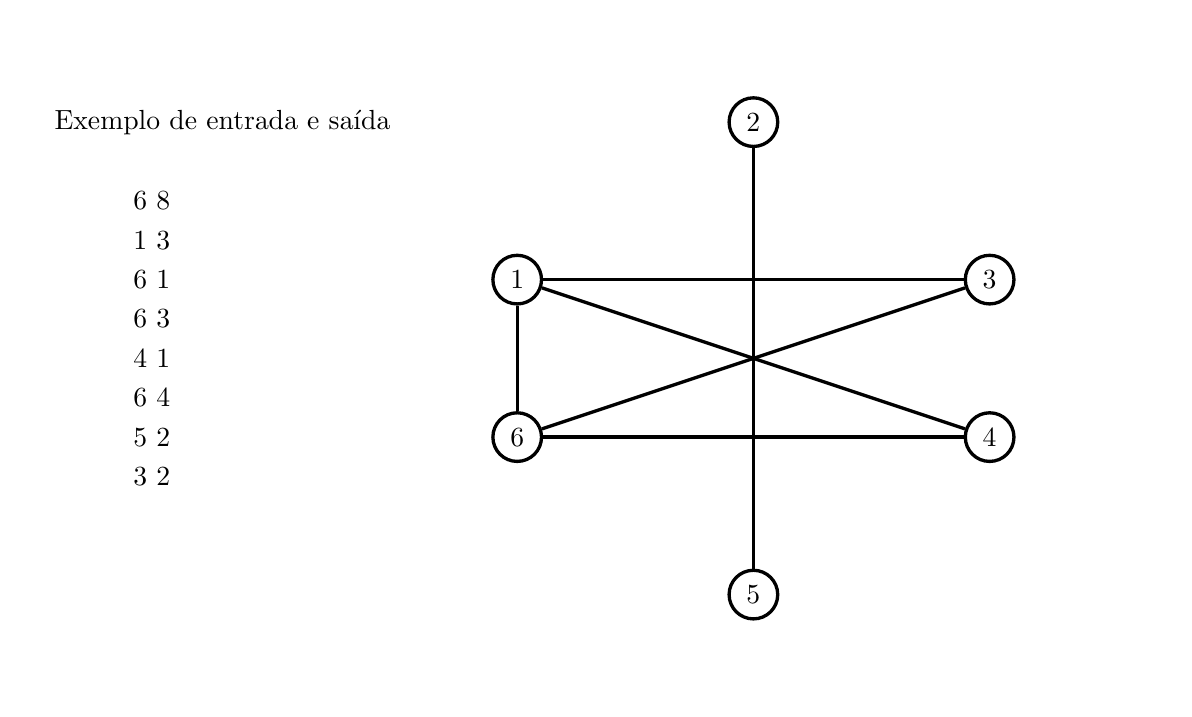
\begin{tikzpicture}
\node[draw,opacity=0] at (0, 0) {x};
\node[draw,opacity=0] at (14, 8) {x};
 \node[anchor=west] at (0, 7) { \bbbold{Exemplo de entrada e saída} };
 \node[anchor=west] at (1, 6) { \bbtext{6 8} };
 \node[circle,draw,very thick] (A) at (6, 5) { \bbtext{1} };
 \node[circle,draw,very thick] (B) at (9, 7) { \bbtext{2} };
 \node[circle,draw,very thick] (C) at (12, 5) { \bbtext{3} };
 \node[circle,draw,very thick] (D) at (12, 3) { \bbtext{4} };
 \node[circle,draw,very thick] (E) at (9, 1) { \bbtext{5} };
 \node[circle,draw,very thick] (F) at (6, 3) { \bbtext{6} };
 \node[anchor=west] at (1, 5.5) { \bbtext{1 3} };
 \draw[very thick] (A) to (C);
 \node[anchor=west] at (1, 5.0) { \bbtext{6 1} };
 \draw[very thick] (A) to (F);
 \node[anchor=west] at (1, 4.5) { \bbtext{6 3} };
 \draw[very thick] (F) to (C);
 \node[anchor=west] at (1, 4.0) { \bbtext{4 1} };
 \draw[very thick] (A) to (D);
 \node[anchor=west] at (1, 3.5) { \bbtext{6 4} };
 \draw[very thick] (D) to (F);
 \node[anchor=west] at (1, 3.0) { \bbtext{5 2} };
 \draw[very thick] (B) to (E);
 \node[anchor=west] at (1, 2.5) { \bbtext{3 2} };
\end{tikzpicture}
\end{frame}

\begin{frame}[plain,t]
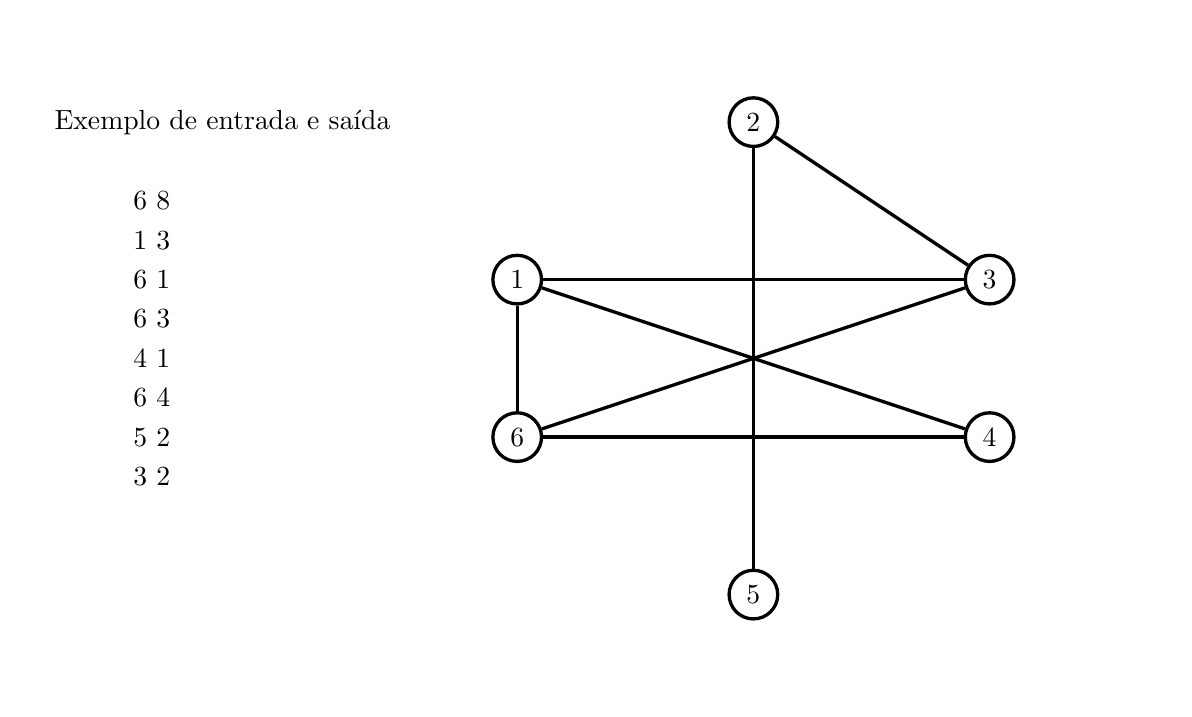
\begin{tikzpicture}
\node[draw,opacity=0] at (0, 0) {x};
\node[draw,opacity=0] at (14, 8) {x};
 \node[anchor=west] at (0, 7) { \bbbold{Exemplo de entrada e saída} };
 \node[anchor=west] at (1, 6) { \bbtext{6 8} };
 \node[circle,draw,very thick] (A) at (6, 5) { \bbtext{1} };
 \node[circle,draw,very thick] (B) at (9, 7) { \bbtext{2} };
 \node[circle,draw,very thick] (C) at (12, 5) { \bbtext{3} };
 \node[circle,draw,very thick] (D) at (12, 3) { \bbtext{4} };
 \node[circle,draw,very thick] (E) at (9, 1) { \bbtext{5} };
 \node[circle,draw,very thick] (F) at (6, 3) { \bbtext{6} };
 \node[anchor=west] at (1, 5.5) { \bbtext{1 3} };
 \draw[very thick] (A) to (C);
 \node[anchor=west] at (1, 5.0) { \bbtext{6 1} };
 \draw[very thick] (A) to (F);
 \node[anchor=west] at (1, 4.5) { \bbtext{6 3} };
 \draw[very thick] (F) to (C);
 \node[anchor=west] at (1, 4.0) { \bbtext{4 1} };
 \draw[very thick] (A) to (D);
 \node[anchor=west] at (1, 3.5) { \bbtext{6 4} };
 \draw[very thick] (D) to (F);
 \node[anchor=west] at (1, 3.0) { \bbtext{5 2} };
 \draw[very thick] (B) to (E);
 \node[anchor=west] at (1, 2.5) { \bbtext{3 2} };
 \draw[very thick] (B) to (C);
\end{tikzpicture}
\end{frame}

\begin{frame}[plain,t]
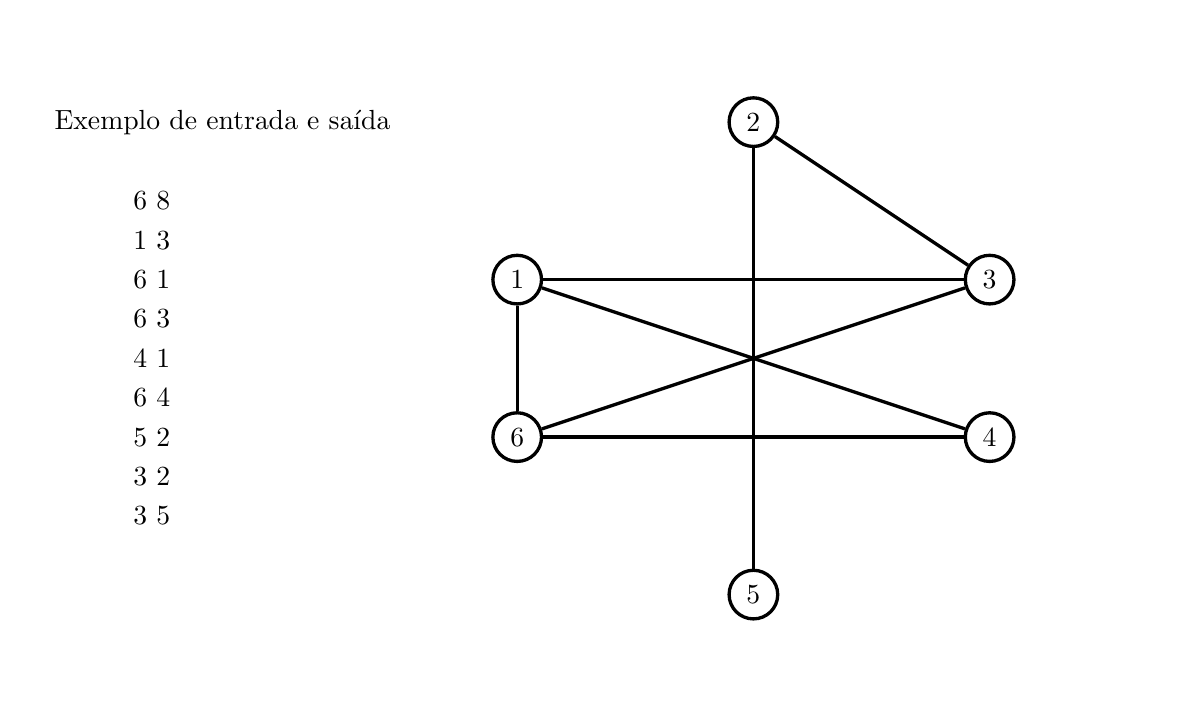
\begin{tikzpicture}
\node[draw,opacity=0] at (0, 0) {x};
\node[draw,opacity=0] at (14, 8) {x};
 \node[anchor=west] at (0, 7) { \bbbold{Exemplo de entrada e saída} };
 \node[anchor=west] at (1, 6) { \bbtext{6 8} };
 \node[circle,draw,very thick] (A) at (6, 5) { \bbtext{1} };
 \node[circle,draw,very thick] (B) at (9, 7) { \bbtext{2} };
 \node[circle,draw,very thick] (C) at (12, 5) { \bbtext{3} };
 \node[circle,draw,very thick] (D) at (12, 3) { \bbtext{4} };
 \node[circle,draw,very thick] (E) at (9, 1) { \bbtext{5} };
 \node[circle,draw,very thick] (F) at (6, 3) { \bbtext{6} };
 \node[anchor=west] at (1, 5.5) { \bbtext{1 3} };
 \draw[very thick] (A) to (C);
 \node[anchor=west] at (1, 5.0) { \bbtext{6 1} };
 \draw[very thick] (A) to (F);
 \node[anchor=west] at (1, 4.5) { \bbtext{6 3} };
 \draw[very thick] (F) to (C);
 \node[anchor=west] at (1, 4.0) { \bbtext{4 1} };
 \draw[very thick] (A) to (D);
 \node[anchor=west] at (1, 3.5) { \bbtext{6 4} };
 \draw[very thick] (D) to (F);
 \node[anchor=west] at (1, 3.0) { \bbtext{5 2} };
 \draw[very thick] (B) to (E);
 \node[anchor=west] at (1, 2.5) { \bbtext{3 2} };
 \draw[very thick] (B) to (C);
 \node[anchor=west] at (1, 2.0) { \bbtext{3 5} };
\end{tikzpicture}
\end{frame}

\begin{frame}[plain,t]
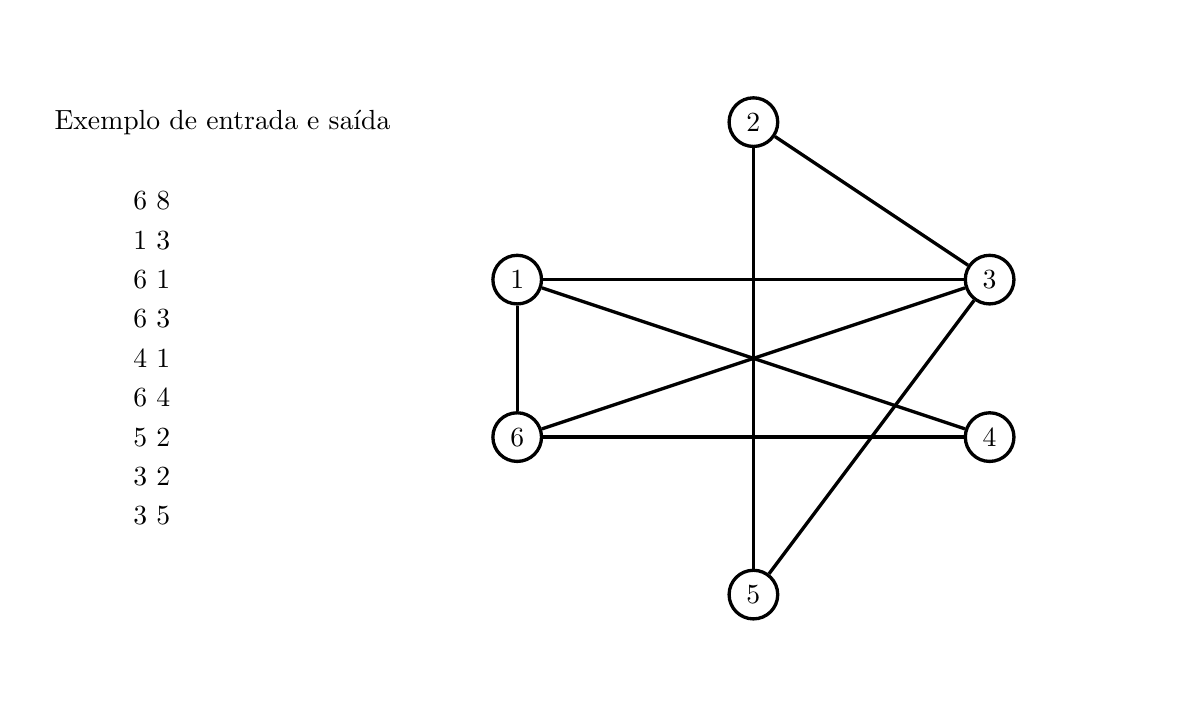
\begin{tikzpicture}
\node[draw,opacity=0] at (0, 0) {x};
\node[draw,opacity=0] at (14, 8) {x};
 \node[anchor=west] at (0, 7) { \bbbold{Exemplo de entrada e saída} };
 \node[anchor=west] at (1, 6) { \bbtext{6 8} };
 \node[circle,draw,very thick] (A) at (6, 5) { \bbtext{1} };
 \node[circle,draw,very thick] (B) at (9, 7) { \bbtext{2} };
 \node[circle,draw,very thick] (C) at (12, 5) { \bbtext{3} };
 \node[circle,draw,very thick] (D) at (12, 3) { \bbtext{4} };
 \node[circle,draw,very thick] (E) at (9, 1) { \bbtext{5} };
 \node[circle,draw,very thick] (F) at (6, 3) { \bbtext{6} };
 \node[anchor=west] at (1, 5.5) { \bbtext{1 3} };
 \draw[very thick] (A) to (C);
 \node[anchor=west] at (1, 5.0) { \bbtext{6 1} };
 \draw[very thick] (A) to (F);
 \node[anchor=west] at (1, 4.5) { \bbtext{6 3} };
 \draw[very thick] (F) to (C);
 \node[anchor=west] at (1, 4.0) { \bbtext{4 1} };
 \draw[very thick] (A) to (D);
 \node[anchor=west] at (1, 3.5) { \bbtext{6 4} };
 \draw[very thick] (D) to (F);
 \node[anchor=west] at (1, 3.0) { \bbtext{5 2} };
 \draw[very thick] (B) to (E);
 \node[anchor=west] at (1, 2.5) { \bbtext{3 2} };
 \draw[very thick] (B) to (C);
 \node[anchor=west] at (1, 2.0) { \bbtext{3 5} };
 \draw[very thick] (E) to (C);
\end{tikzpicture}
\end{frame}

\begin{frame}[plain,t]
\begin{tikzpicture}
\node[draw,opacity=0] at (0, 0) {x};
\node[draw,opacity=0] at (14, 8) {x};
 \node[anchor=west] at (0, 7) { \bbbold{Exemplo de entrada e saída} };
 \node[anchor=west] at (1, 6) { \bbtext{6 8} };
 \node[circle,draw,very thick] (A) at (6, 5) { \bbtext{1} };
 \node[circle,draw,very thick] (B) at (9, 7) { \bbtext{2} };
 \node[circle,draw,very thick] (D) at (12, 3) { \bbtext{4} };
 \node[circle,draw,very thick] (E) at (9, 1) { \bbtext{5} };
 \node[circle,draw,very thick] (F) at (6, 3) { \bbtext{6} };
 \node[anchor=west] at (1, 5.5) { \bbtext{1 3} };
 \draw[very thick] (A) to (C);
 \node[anchor=west] at (1, 5.0) { \bbtext{6 1} };
 \draw[very thick] (A) to (F);
 \node[anchor=west] at (1, 4.5) { \bbtext{6 3} };
 \draw[very thick] (F) to (C);
 \node[anchor=west] at (1, 4.0) { \bbtext{4 1} };
 \draw[very thick] (A) to (D);
 \node[anchor=west] at (1, 3.5) { \bbtext{6 4} };
 \draw[very thick] (D) to (F);
 \node[anchor=west] at (1, 3.0) { \bbtext{5 2} };
 \draw[very thick] (B) to (E);
 \node[anchor=west] at (1, 2.5) { \bbtext{3 2} };
 \draw[very thick] (B) to (C);
 \node[anchor=west] at (1, 2.0) { \bbtext{3 5} };
 \draw[very thick] (E) to (C);
 \node[circle,fill,color=BBRed] (C) at (12, 5) { \bbtext{3} };
 \node[circle,draw,very thick] (C) at (12, 5) { \bbtext{3} };
\end{tikzpicture}
\end{frame}

\begin{frame}[plain,t]
\begin{tikzpicture}
\node[draw,opacity=0] at (0, 0) {x};
\node[draw,opacity=0] at (14, 8) {x};
 \node[anchor=west] at (0, 7) { \bbbold{Exemplo de entrada e saída} };
 \node[anchor=west] at (1, 6) { \bbtext{6 8} };
 \node[circle,draw,very thick] (A) at (6, 5) { \bbtext{1} };
 \node[circle,draw,very thick] (B) at (9, 7) { \bbtext{2} };
 \node[circle,draw,very thick] (D) at (12, 3) { \bbtext{4} };
 \node[circle,draw,very thick] (E) at (9, 1) { \bbtext{5} };
 \node[circle,draw,very thick] (F) at (6, 3) { \bbtext{6} };
 \node[anchor=west] at (1, 5.5) { \bbtext{1 3} };
 \node[anchor=west] at (1, 5.0) { \bbtext{6 1} };
 \draw[very thick] (A) to (F);
 \node[anchor=west] at (1, 4.5) { \bbtext{6 3} };
 \node[anchor=west] at (1, 4.0) { \bbtext{4 1} };
 \draw[very thick] (A) to (D);
 \node[anchor=west] at (1, 3.5) { \bbtext{6 4} };
 \draw[very thick] (D) to (F);
 \node[anchor=west] at (1, 3.0) { \bbtext{5 2} };
 \draw[very thick] (B) to (E);
 \node[anchor=west] at (1, 2.5) { \bbtext{3 2} };
 \node[anchor=west] at (1, 2.0) { \bbtext{3 5} };
\end{tikzpicture}
\end{frame}

\begin{frame}[plain,t]
\begin{tikzpicture}
\node[draw,opacity=0] at (0, 0) {x};
\node[draw,opacity=0] at (14, 8) {x};
 \node[anchor=west] at (0, 7) { \bbbold{Exemplo de entrada e saída} };
 \node[anchor=west] at (1, 6) { \bbtext{6 8} };
 \node[anchor=west] at (1, 5.5) { \bbtext{1 3} };
 \node[anchor=west] at (1, 5.0) { \bbtext{6 1} };
 \draw[very thick] (A) to (F);
 \node[anchor=west] at (1, 4.5) { \bbtext{6 3} };
 \node[anchor=west] at (1, 4.0) { \bbtext{4 1} };
 \draw[very thick] (A) to (D);
 \node[anchor=west] at (1, 3.5) { \bbtext{6 4} };
 \draw[very thick] (D) to (F);
 \node[anchor=west] at (1, 3.0) { \bbtext{5 2} };
 \draw[very thick] (B) to (E);
 \node[anchor=west] at (1, 2.5) { \bbtext{3 2} };
 \node[anchor=west] at (1, 2.0) { \bbtext{3 5} };
 \node[circle,fill,color=BBCyan] (A) at (6, 5) { \bbtext{1} };
 \node[circle,draw,very thick] (A) at (6, 5) { \bbtext{1} };
 \node[circle,fill,color=BBGreen] (B) at (9, 7) { \bbtext{2} };
 \node[circle,draw,very thick] (B) at (9, 7) { \bbtext{2} };
 \node[circle,fill,color=BBCyan] (D) at (12, 3) { \bbtext{4} };
 \node[circle,draw,very thick] (D) at (12, 3) { \bbtext{4} };
 \node[circle,fill,color=BBGreen] (E) at (9, 1) { \bbtext{5} };
 \node[circle,draw,very thick] (E) at (9, 1) { \bbtext{5} };
 \node[circle,fill,color=BBCyan] (F) at (6, 3) { \bbtext{6} };
 \node[circle,draw,very thick] (F) at (6, 3) { \bbtext{6} };
\end{tikzpicture}
\end{frame}

\begin{frame}[plain,t]
\begin{tikzpicture}
\node[draw,opacity=0] at (0, 0) {x};
\node[draw,opacity=0] at (14, 8) {x};
 \node[anchor=west] at (0, 7) { \bbbold{Exemplo de entrada e saída} };
 \node[anchor=west] at (1, 6) { \bbtext{6 8} };
 \node[anchor=west] at (1, 5.5) { \bbtext{1 3} };
 \node[anchor=west] at (1, 5.0) { \bbtext{6 1} };
 \draw[very thick] (A) to (F);
 \node[anchor=west] at (1, 4.5) { \bbtext{6 3} };
 \node[anchor=west] at (1, 4.0) { \bbtext{4 1} };
 \draw[very thick] (A) to (D);
 \node[anchor=west] at (1, 3.5) { \bbtext{6 4} };
 \draw[very thick] (D) to (F);
 \node[anchor=west] at (1, 3.0) { \bbtext{5 2} };
 \draw[very thick] (B) to (E);
 \node[anchor=west] at (1, 2.5) { \bbtext{3 2} };
 \node[anchor=west] at (1, 2.0) { \bbtext{3 5} };
 \node[circle,fill,color=BBCyan] (A) at (6, 5) { \bbtext{1} };
 \node[circle,draw,very thick] (A) at (6, 5) { \bbtext{1} };
 \node[circle,fill,color=BBGreen] (B) at (9, 7) { \bbtext{2} };
 \node[circle,draw,very thick] (B) at (9, 7) { \bbtext{2} };
 \node[circle,fill,color=BBCyan] (D) at (12, 3) { \bbtext{4} };
 \node[circle,draw,very thick] (D) at (12, 3) { \bbtext{4} };
 \node[circle,fill,color=BBGreen] (E) at (9, 1) { \bbtext{5} };
 \node[circle,draw,very thick] (E) at (9, 1) { \bbtext{5} };
 \node[circle,fill,color=BBCyan] (F) at (6, 3) { \bbtext{6} };
 \node[circle,draw,very thick] (F) at (6, 3) { \bbtext{6} };
 \draw[-latex,very thick] (1.4, 0.8) to (1.4, 1.8);
 \node at (1.4, 0.5) { \bbinfo{1} };
\end{tikzpicture}
\end{frame}

\begin{frame}[plain,t]
\begin{tikzpicture}
\node[draw,opacity=0] at (0, 0) {x};
\node[draw,opacity=0] at (14, 8) {x};
 \node[anchor=west] at (0, 7) { \bbbold{Exemplo de entrada e saída} };
 \node[anchor=west] at (1, 6) { \bbtext{6 8} };
 \node[anchor=west] at (1, 5.5) { \bbtext{1 3} };
 \node[anchor=west] at (1, 5.0) { \bbtext{6 1} };
 \draw[very thick] (A) to (F);
 \node[anchor=west] at (1, 4.5) { \bbtext{6 3} };
 \node[anchor=west] at (1, 4.0) { \bbtext{4 1} };
 \draw[very thick] (A) to (D);
 \node[anchor=west] at (1, 3.5) { \bbtext{6 4} };
 \draw[very thick] (D) to (F);
 \node[anchor=west] at (1, 3.0) { \bbtext{5 2} };
 \draw[very thick] (B) to (E);
 \node[anchor=west] at (1, 2.5) { \bbtext{3 2} };
 \node[anchor=west] at (1, 2.0) { \bbtext{3 5} };
 \node[circle,fill,color=BBCyan] (A) at (6, 5) { \bbtext{1} };
 \node[circle,draw,very thick] (A) at (6, 5) { \bbtext{1} };
 \node[circle,fill,color=BBGreen] (B) at (9, 7) { \bbtext{2} };
 \node[circle,draw,very thick] (B) at (9, 7) { \bbtext{2} };
 \node[circle,fill,color=BBCyan] (D) at (12, 3) { \bbtext{4} };
 \node[circle,draw,very thick] (D) at (12, 3) { \bbtext{4} };
 \node[circle,fill,color=BBGreen] (E) at (9, 1) { \bbtext{5} };
 \node[circle,draw,very thick] (E) at (9, 1) { \bbtext{5} };
 \node[circle,fill,color=BBCyan] (F) at (6, 3) { \bbtext{6} };
 \node[circle,draw,very thick] (F) at (6, 3) { \bbtext{6} };
 \draw[-latex,very thick] (1.4, 0.8) to (1.4, 1.8);
 \node at (1.4, 0.5) { \bbinfo{1} };
\end{tikzpicture}
\end{frame}

\begin{frame}[plain,t]
\begin{tikzpicture}
\node[draw,opacity=0] at (0, 0) {x};
\node[draw,opacity=0] at (14, 8) {x};
 \node[anchor=west] at (0, 6) { \Large \bbbold{Solução} };
\end{tikzpicture}
\end{frame}

\begin{frame}[plain,t]
\begin{tikzpicture}
\node[draw,opacity=0] at (0, 0) {x};
\node[draw,opacity=0] at (14, 8) {x};
 \node[anchor=west] at (0, 6) { \Large \bbbold{Solução} };
 \node[anchor=west] at (1, 5) { \bbtext{Basta contar os pontos de articulação!} };
\end{tikzpicture}
\end{frame}

\begin{frame}[plain,t]
 \inputsnippet{cpp}{11}{30}{codes/SUBMERGE.cpp}
\end{frame}

\begin{frame}[plain,t]
 \inputsnippet{cpp}{32}{49}{codes/SUBMERGE.cpp}
\end{frame}

\end{document}
